\documentclass[22pt]{beamer}

\usepackage{templates/beamerthemekit}
\usepackage{graphicx}
\usepackage[utf8]{inputenc}
\usepackage[ngerman]{babel}

\title[OSIP]{OPC UA Simulator for Industrial Plants}
\subtitle{PSE Projekt}
\author{M. Armbruster, D. Kahles, H. Lehmann, M. Schwarzmann, N. Wilhelm}

\titlelogo{icon}

\begin{document}

\selectlanguage{ngerman}

%title page
\begin{frame}
\titlepage
\end{frame}

\begin{frame}{Wofür benötigt man OSIP?}
\begin{figure}[ht!]
\centering
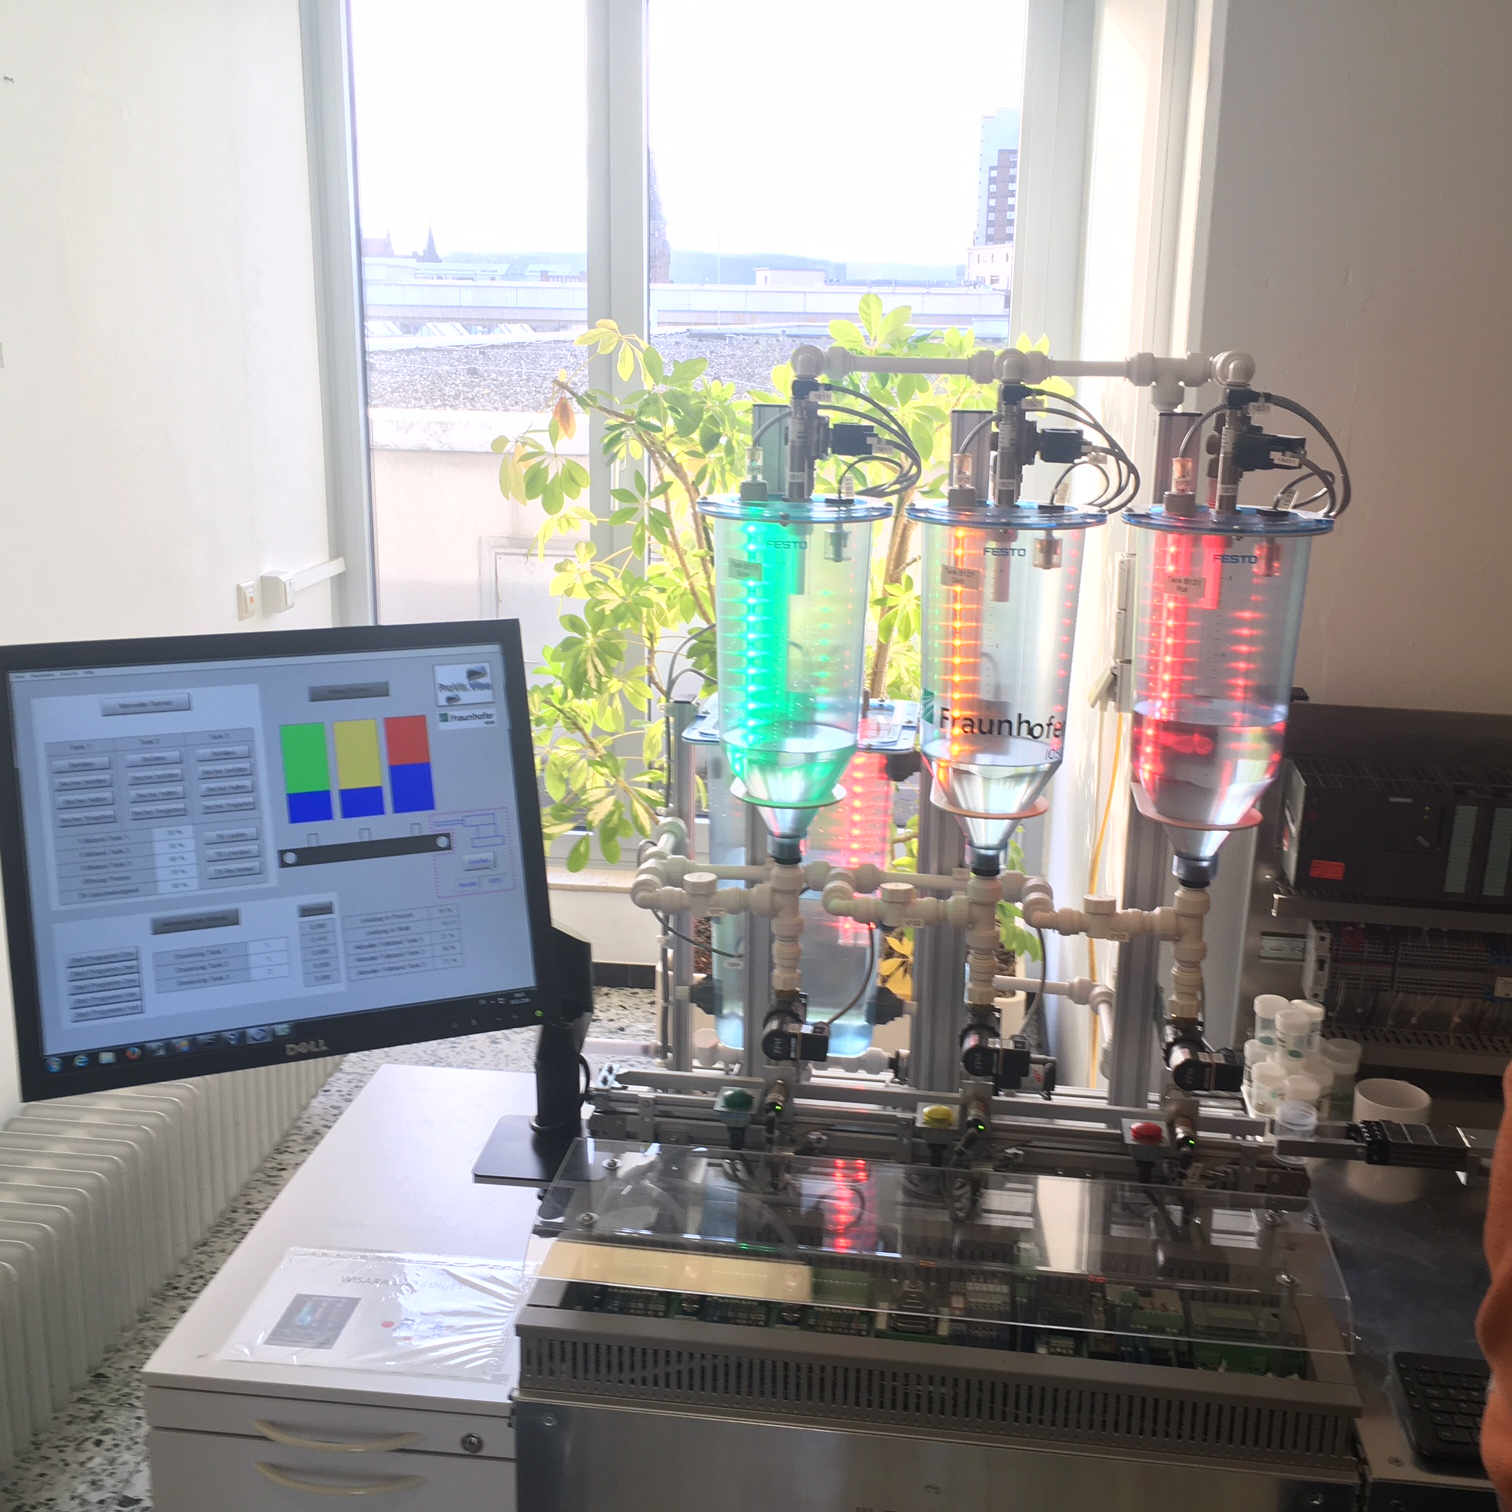
\includegraphics[height=\textheight,width=\textwidth,keepaspectratio=true]{Demoanlage_IOSB.jpg}
\end{figure}
\end{frame}

\begin{frame}{Was ist OSIP?}
\begin{itemize}[<+->]
 \item Besteht aus zwei Anwendungen: Die \emph{Simulation} eines chemischen Produktionsprozesses mit vier Tanks und die \emph{Überwachungskonsole}
 \item Kommunikation ausschließlich über OPC UA Protokoll
 \item Anwendungen auf getrennten Computern lauffähig, sofern Netzwerkverbindung besteht
\end{itemize}
\end{frame}

\begin{frame}{Simulation}
 \begin{itemize}[<+->]
  \item Drei Tanks mit Flüssigkeiten die in einem Mischtank gemischt werden
  \item Verschiedene Parameter einstellbar (Ventile, Einflusstemperaturen, ...)
  \item Komponenten der Anlage werden schematisch dargestellt
  \item Flüssigkeiten werden physikalisch korrekt simuliert
  \item Enthält für jeden Tank einen eigenen OPC UA Server mit konfigurierbaren Ports
  \item OPC UA Server stellen verschiedene Sensorwerte bereit (Füllstände, Temperaturen, Alarmzustände, ...)
  \item Mit Szenarien können interessante Abläufe automatisiert werden
 \end{itemize}
\end{frame}

\begin{frame}{Überwachungskonsole}
 \begin{itemize}[<+->]
  \item Erhält per OPC UA Messwerte der Simulation und visualisiert diese
  \item Nimmt keinen Einfluss auf die Simulation, reines Monitoring
  \item Fragt Sensorwerte in einstellbarem Intervall von den OPC UA Servern ab
  \item Warnt beim Überschreiten von definierten Grenzen den Benutzer
  \item Alarme sind unabhängig vom Aktualisierungsintervall
  \item Alarme sind ein- und ausschaltbar
  \item Eine Loggingkonsole zeigt Alarme und Fehler an
 \end{itemize}
\end{frame}

\begin{frame}{Verwendete Technologien}
\begin{itemize}[<+->]
 \item OPC UA Protokoll wird nicht selbst implementiert $\rightarrow$ Open Source Implementierung \emph{Milo}
 \item OSIP wird in \emph{Java} entwickelt
 \item Die GUI wird mit \emph{JavaFX} implementiert
 \item \emph{Git} (circa 800 Commits) mit Codereview auf \emph{GitHub.com}
 \item Lauffähig auf Ubuntu 16.04 und Windows 10
 \item Unter Ubuntu: einfaches starten in Docker Containern
 \item Verschiedene Entwurfsmuster verwendet (MVC, Beobachter, Fassade, Strategie, ...)
 \item Circa 15.000 LOC, davon 7500 SLOC
\end{itemize}
\end{frame}

\begin{frame}{Resümee}
\begin{itemize}[<+->]
 \item Code Review vermeidet viele Probleme
 \item Controller aufwändiger als gedacht
 \item Unittesten der Nicht-GUI Komponenten nützlich
 \item Zeitplan dank Puffer bisher eingehalten
 \item Alle geplanten Features sind umgesetzt
\end{itemize}
\end{frame}

\end{document}
